\section{CThread\-Recursive\-Mutex  Class Reference}
\label{classCThreadRecursiveMutex}\index{CThreadRecursiveMutex@{CThread\-Recursive\-Mutex}}
CThread\-Recursive\-Mutex {\bf CThread\-Recursive\-Mutex.h}. 


{\tt \#include $<$CThread\-Recursive\-Mutex.h$>$}

Inheritance diagram for CThread\-Recursive\-Mutex::\begin{figure}[H]
\begin{center}
\leavevmode
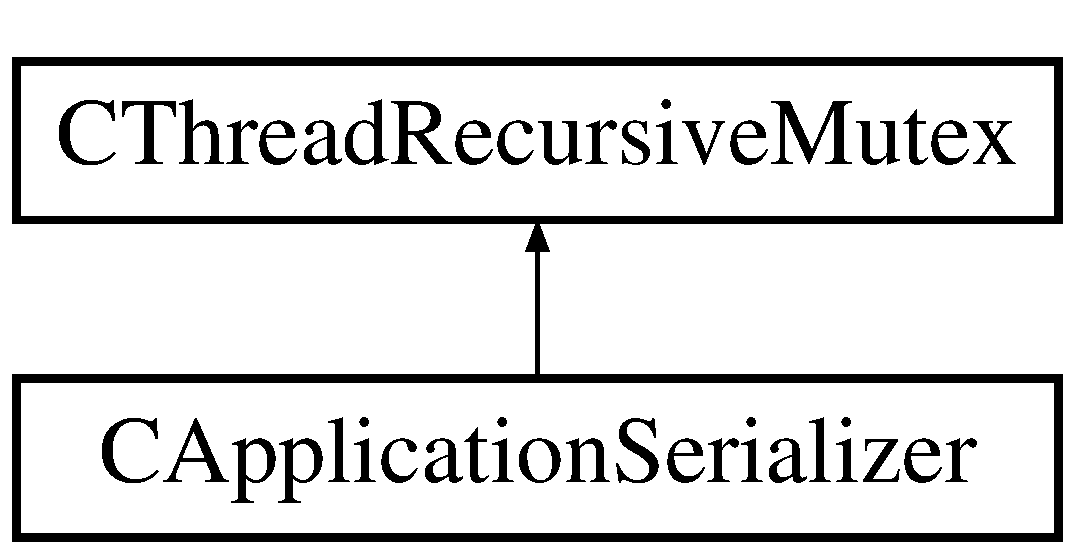
\includegraphics[height=2cm]{classCThreadRecursiveMutex}
\end{center}
\end{figure}
\subsection*{Public Methods}
\begin{CompactItemize}
\item 
{\bf CThread\-Recursive\-Mutex} ()
\begin{CompactList}\small\item\em Default Constructor.\item\end{CompactList}\item 
{\bf $\sim$CThread\-Recursive\-Mutex} ()
\begin{CompactList}\small\item\em Destructor.\item\end{CompactList}\item 
DAQThread\-Mutex {\bf get\-Mutex} () const
\begin{CompactList}\small\item\em $<$ Retrieve m\_\-Mutex.\item\end{CompactList}\item 
daqthread\_\-t {\bf get\-Owning\-Thread} () const
\begin{CompactList}\small\item\em $<$ Retrieve m\_\-t\-Owning\-Thread.\item\end{CompactList}\item 
unsigned {\bf get\-Lock\-Level} () const
\begin{CompactList}\small\item\em $<$ Retrieve m\_\-Lock\-Level.\item\end{CompactList}\item 
DAQThread\-Mutex {\bf get\-Monitor\-Mutex} () const
\begin{CompactList}\small\item\em $<$ Return m\_\-Monito\-Mutex.\item\end{CompactList}\item 
int {\bf Lock} ()
\item 
int {\bf Un\-Lock} ()
\item 
int {\bf Try\-Lock} ()
\item 
int {\bf is\-Locked} ()
\item 
void {\bf Un\-Lock\-Completely} ()
\end{CompactItemize}
\subsection*{Protected Methods}
\begin{CompactItemize}
\item 
void {\bf set\-Mutex} (const DAQThread\-Mutex am\_\-Mutex)
\item 
void {\bf set\-Owning\-Thread} (const daqthread\_\-t am\_\-t\-Owning\-Thread)
\item 
void {\bf set\-Lock\-Level} (const unsigned am\_\-n\-Lock\-Level)
\item 
void {\bf set\-Monitor\-Mutex} (const DAQThread\-Mutex am\_\-Monitor\-Mutex)
\end{CompactItemize}
\subsection*{Private Methods}
\begin{CompactItemize}
\item 
{\bf CThread\-Recursive\-Mutex} (const CThread\-Recursive\-Mutex \&r\-Rhs)
\item 
int {\bf operator==} (const CThread\-Recursive\-Mutex \&a\-CThread\-Recursive\-Mutex) const
\end{CompactItemize}
\subsection*{Private Attributes}
\begin{CompactItemize}
\item 
DAQThread\-Mutex {\bf m\_\-Mutex}
\begin{CompactList}\small\item\em Mutex locked.\item\end{CompactList}\item 
daqthread\_\-t {\bf m\_\-t\-Owning\-Thread}
\begin{CompactList}\small\item\em Id of owning thread.\item\end{CompactList}\item 
unsigned {\bf m\_\-n\-Lock\-Level}
\begin{CompactList}\small\item\em Locking depth for owning thread.\item\end{CompactList}\item 
DAQThread\-Mutex {\bf m\_\-Monitor\-Mutex}
\begin{CompactList}\small\item\em Atomicity Mutex.\item\end{CompactList}\end{CompactItemize}


\subsection{Detailed Description}
CThread\-Recursive\-Mutex {\bf CThread\-Recursive\-Mutex.h}.

Provides a mutex which can be locked in a nested manner by a thread. The \char`\"{}nested ness' is managed through the m\_\-n\-Lock\-Level and the  m\_\-Owning\-Thread member. Atomicity of the otherwise non-atomic  function is handled by bracketing calls with locks of the mutexe's own m\_\-Monitor\-Mutex Gaurentees:\begin{CompactItemize}
\item 
No process will be starved.\item 
Processes blocked waiting for the mutex will be served in the order in which they entered the blocking queue. \end{CompactItemize}




Definition at line 313 of file CThread\-Recursive\-Mutex.h.

\subsection{Constructor \& Destructor Documentation}
\index{CThreadRecursiveMutex@{CThread\-Recursive\-Mutex}!CThreadRecursiveMutex@{CThreadRecursiveMutex}}
\index{CThreadRecursiveMutex@{CThreadRecursiveMutex}!CThreadRecursiveMutex@{CThread\-Recursive\-Mutex}}
\subsubsection{\setlength{\rightskip}{0pt plus 5cm}CThread\-Recursive\-Mutex::CThread\-Recursive\-Mutex ()}\label{classCThreadRecursiveMutex_a0}


Default Constructor.



Definition at line 304 of file CThread\-Recursive\-Mutex.cpp.\index{CThreadRecursiveMutex@{CThread\-Recursive\-Mutex}!~CThreadRecursiveMutex@{$\sim$CThreadRecursiveMutex}}
\index{~CThreadRecursiveMutex@{$\sim$CThreadRecursiveMutex}!CThreadRecursiveMutex@{CThread\-Recursive\-Mutex}}
\subsubsection{\setlength{\rightskip}{0pt plus 5cm}CThread\-Recursive\-Mutex::$\sim$CThread\-Recursive\-Mutex ()}\label{classCThreadRecursiveMutex_a1}


Destructor.



Definition at line 315 of file CThread\-Recursive\-Mutex.cpp.

References m\_\-Monitor\-Mutex, m\_\-Mutex, and m\_\-n\-Lock\-Level.\index{CThreadRecursiveMutex@{CThread\-Recursive\-Mutex}!CThreadRecursiveMutex@{CThreadRecursiveMutex}}
\index{CThreadRecursiveMutex@{CThreadRecursiveMutex}!CThreadRecursiveMutex@{CThread\-Recursive\-Mutex}}
\subsubsection{\setlength{\rightskip}{0pt plus 5cm}CThread\-Recursive\-Mutex::CThread\-Recursive\-Mutex (const CThread\-Recursive\-Mutex \& {\em r\-Rhs})\hspace{0.3cm}{\tt  [private]}}\label{classCThreadRecursiveMutex_c0}


Copy construction is illegal and hence private and not implemented. 

\subsection{Member Function Documentation}
\index{CThreadRecursiveMutex@{CThread\-Recursive\-Mutex}!getLockLevel@{getLockLevel}}
\index{getLockLevel@{getLockLevel}!CThreadRecursiveMutex@{CThread\-Recursive\-Mutex}}
\subsubsection{\setlength{\rightskip}{0pt plus 5cm}unsigned CThread\-Recursive\-Mutex::get\-Lock\-Level () const\hspace{0.3cm}{\tt  [inline]}}\label{classCThreadRecursiveMutex_a4}


$<$ Retrieve m\_\-Lock\-Level.



Definition at line 352 of file CThread\-Recursive\-Mutex.h.

References m\_\-n\-Lock\-Level.

Referenced by CEvent::Disable().\index{CThreadRecursiveMutex@{CThread\-Recursive\-Mutex}!getMonitorMutex@{getMonitorMutex}}
\index{getMonitorMutex@{getMonitorMutex}!CThreadRecursiveMutex@{CThread\-Recursive\-Mutex}}
\subsubsection{\setlength{\rightskip}{0pt plus 5cm}DAQThread\-Mutex CThread\-Recursive\-Mutex::get\-Monitor\-Mutex () const\hspace{0.3cm}{\tt  [inline]}}\label{classCThreadRecursiveMutex_a5}


$<$ Return m\_\-Monito\-Mutex.



Definition at line 356 of file CThread\-Recursive\-Mutex.h.

References m\_\-Monitor\-Mutex.\index{CThreadRecursiveMutex@{CThread\-Recursive\-Mutex}!getMutex@{getMutex}}
\index{getMutex@{getMutex}!CThreadRecursiveMutex@{CThread\-Recursive\-Mutex}}
\subsubsection{\setlength{\rightskip}{0pt plus 5cm}DAQThread\-Mutex CThread\-Recursive\-Mutex::get\-Mutex () const\hspace{0.3cm}{\tt  [inline]}}\label{classCThreadRecursiveMutex_a2}


$<$ Retrieve m\_\-Mutex.



Definition at line 344 of file CThread\-Recursive\-Mutex.h.

References m\_\-Mutex.\index{CThreadRecursiveMutex@{CThread\-Recursive\-Mutex}!getOwningThread@{getOwningThread}}
\index{getOwningThread@{getOwningThread}!CThreadRecursiveMutex@{CThread\-Recursive\-Mutex}}
\subsubsection{\setlength{\rightskip}{0pt plus 5cm}daqthread\_\-t CThread\-Recursive\-Mutex::get\-Owning\-Thread () const\hspace{0.3cm}{\tt  [inline]}}\label{classCThreadRecursiveMutex_a3}


$<$ Retrieve m\_\-t\-Owning\-Thread.



Definition at line 348 of file CThread\-Recursive\-Mutex.h.

References m\_\-t\-Owning\-Thread.

Referenced by CEvent::Disable().\index{CThreadRecursiveMutex@{CThread\-Recursive\-Mutex}!isLocked@{isLocked}}
\index{isLocked@{isLocked}!CThreadRecursiveMutex@{CThread\-Recursive\-Mutex}}
\subsubsection{\setlength{\rightskip}{0pt plus 5cm}int CThread\-Recursive\-Mutex::is\-Locked ()}\label{classCThreadRecursiveMutex_a9}


Operation Type: Override.

Purpose:

Returns non zero if someone, anyone (even self()) owns the mutex. Note that the mutex is considered owned if the lock level is  nonzero. This should even be faster than the base class  implementation. 

Definition at line 488 of file CThread\-Recursive\-Mutex.cpp.

References m\_\-Monitor\-Mutex, and m\_\-n\-Lock\-Level.\index{CThreadRecursiveMutex@{CThread\-Recursive\-Mutex}!Lock@{Lock}}
\index{Lock@{Lock}!CThreadRecursiveMutex@{CThread\-Recursive\-Mutex}}
\subsubsection{\setlength{\rightskip}{0pt plus 5cm}int CThread\-Recursive\-Mutex::Lock ()}\label{classCThreadRecursiveMutex_a6}


Operation Type: Override.

Purpose:

Locks the mutex. Returns zero on success, otherwise, errno has the reason for the failure. Note that if we own the mutex the lock level is incremented, otherwise, this function may block. 

Definition at line 341 of file CThread\-Recursive\-Mutex.cpp.

References m\_\-Monitor\-Mutex, m\_\-Mutex, m\_\-n\-Lock\-Level, and m\_\-t\-Owning\-Thread.

Referenced by CBuffer\-Event$<$ T $>$::Add\-Link(), CSocket::Address\-To\-Host\-String(), CSocket::Connect(), CBuffer\-Event$<$ T $>$::Delete\-Link(), CDAQTCLProcessor::Delete\-Relay(), CEvent::Disable(), CEvent::Enable(), CDAQTCLProcessor::Eval\-Relay(), CBuffer\-Event$<$ U $>$::get\-Pending\-Add\-Queue(), CBuffer\-Event$<$ U $>$::get\-Pending\-Delete\-Queue(), CTCPConnection\-Lost::Host(), CEvent::On\-Event(), CSocket::Open\-Socket(), CXt\-Event\-Loop::operator()(), CTCPConnection\-Lost::Port(), CBuffer\-Event$<$ T $>$::Process\-Add\-Queue(), CBuffer\-Event$<$ T $>$::Process\-Del\-Queue(), CServer\-Connection\-Event::Protocol(), and CSocket::Service().\index{CThreadRecursiveMutex@{CThread\-Recursive\-Mutex}!operator==@{operator==}}
\index{operator==@{operator==}!CThreadRecursiveMutex@{CThread\-Recursive\-Mutex}}
\subsubsection{\setlength{\rightskip}{0pt plus 5cm}int CThread\-Recursive\-Mutex::operator== (const CThread\-Recursive\-Mutex \& {\em a\-CThread\-Recursive\-Mutex}) const\hspace{0.3cm}{\tt  [private]}}\label{classCThreadRecursiveMutex_c1}


Assignment is illegal and hence private and not implemented. \index{CThreadRecursiveMutex@{CThread\-Recursive\-Mutex}!setLockLevel@{setLockLevel}}
\index{setLockLevel@{setLockLevel}!CThreadRecursiveMutex@{CThread\-Recursive\-Mutex}}
\subsubsection{\setlength{\rightskip}{0pt plus 5cm}void CThread\-Recursive\-Mutex::set\-Lock\-Level (const unsigned {\em am\_\-n\-Lock\-Level})\hspace{0.3cm}{\tt  [inline, protected]}}\label{classCThreadRecursiveMutex_b2}


\begin{Desc}
\item[Parameters: ]\par
\begin{description}
\item[{\em 
am\_\-n\-Lock\-Level}]Set m\_\-n\-Lock\-Level \end{description}
\end{Desc}


Definition at line 371 of file CThread\-Recursive\-Mutex.h.

References m\_\-n\-Lock\-Level.\index{CThreadRecursiveMutex@{CThread\-Recursive\-Mutex}!setMonitorMutex@{setMonitorMutex}}
\index{setMonitorMutex@{setMonitorMutex}!CThreadRecursiveMutex@{CThread\-Recursive\-Mutex}}
\subsubsection{\setlength{\rightskip}{0pt plus 5cm}void CThread\-Recursive\-Mutex::set\-Monitor\-Mutex (const DAQThread\-Mutex {\em am\_\-Monitor\-Mutex})\hspace{0.3cm}{\tt  [inline, protected]}}\label{classCThreadRecursiveMutex_b3}


\begin{Desc}
\item[Parameters: ]\par
\begin{description}
\item[{\em 
am\_\-Monitor\-Mutex}]Set m\_\-Monitor\-Mutex \end{description}
\end{Desc}


Definition at line 374 of file CThread\-Recursive\-Mutex.h.

References m\_\-Monitor\-Mutex.\index{CThreadRecursiveMutex@{CThread\-Recursive\-Mutex}!setMutex@{setMutex}}
\index{setMutex@{setMutex}!CThreadRecursiveMutex@{CThread\-Recursive\-Mutex}}
\subsubsection{\setlength{\rightskip}{0pt plus 5cm}void CThread\-Recursive\-Mutex::set\-Mutex (const DAQThread\-Mutex {\em am\_\-Mutex})\hspace{0.3cm}{\tt  [inline, protected]}}\label{classCThreadRecursiveMutex_b0}


\begin{Desc}
\item[Parameters: ]\par
\begin{description}
\item[{\em 
am\_\-Mutex}]Set m\_\-Mutex \end{description}
\end{Desc}


Definition at line 365 of file CThread\-Recursive\-Mutex.h.

References m\_\-Mutex.\index{CThreadRecursiveMutex@{CThread\-Recursive\-Mutex}!setOwningThread@{setOwningThread}}
\index{setOwningThread@{setOwningThread}!CThreadRecursiveMutex@{CThread\-Recursive\-Mutex}}
\subsubsection{\setlength{\rightskip}{0pt plus 5cm}void CThread\-Recursive\-Mutex::set\-Owning\-Thread (const daqthread\_\-t {\em am\_\-t\-Owning\-Thread})\hspace{0.3cm}{\tt  [inline, protected]}}\label{classCThreadRecursiveMutex_b1}


\begin{Desc}
\item[Parameters: ]\par
\begin{description}
\item[{\em 
am\_\-t\-Owning\-Thread}]Set m\_\-t\-Owning\-Thread \end{description}
\end{Desc}


Definition at line 368 of file CThread\-Recursive\-Mutex.h.

References m\_\-t\-Owning\-Thread.\index{CThreadRecursiveMutex@{CThread\-Recursive\-Mutex}!TryLock@{TryLock}}
\index{TryLock@{TryLock}!CThreadRecursiveMutex@{CThread\-Recursive\-Mutex}}
\subsubsection{\setlength{\rightskip}{0pt plus 5cm}int CThread\-Recursive\-Mutex::Try\-Lock ()}\label{classCThreadRecursiveMutex_a8}


Operation Type: Override

Purpose:

Tries to lock the mutex.  If the mutex is owned by the running thread the lock succeeds and the lock level is incremented. If the lock level is zero, then trylock is done on the base class and the result is returned. On success, the lock level is incremented. Returns 0 on success, otherwise, errno has reason for failure, if the lock was already held, errno == EAGAIN. 

Definition at line 450 of file CThread\-Recursive\-Mutex.cpp.

References m\_\-Monitor\-Mutex, m\_\-Mutex, m\_\-n\-Lock\-Level, and m\_\-t\-Owning\-Thread.\index{CThreadRecursiveMutex@{CThread\-Recursive\-Mutex}!UnLock@{UnLock}}
\index{UnLock@{UnLock}!CThreadRecursiveMutex@{CThread\-Recursive\-Mutex}}
\subsubsection{\setlength{\rightskip}{0pt plus 5cm}int CThread\-Recursive\-Mutex::Un\-Lock ()}\label{classCThreadRecursiveMutex_a7}


Operation Type: Override

Purpose:

Unlocks a locked mutex. If the mutex is already locked by us, the lock level is decremented. The mutex is not actually released until the lock level goes to zero. If we don't own the mutex, and error results. Returns zero on success, otherwise, errno has the reason for the failure. 

Definition at line 396 of file CThread\-Recursive\-Mutex.cpp.

References m\_\-Monitor\-Mutex, m\_\-Mutex, m\_\-n\-Lock\-Level, and m\_\-t\-Owning\-Thread.

Referenced by CBuffer\-Event$<$ T $>$::Add\-Link(), CSocket::Address\-To\-Host\-String(), CSocket::Connect(), CBuffer\-Event$<$ T $>$::Delete\-Link(), CDAQTCLProcessor::Delete\-Relay(), CEvent::Enable(), CDAQTCLProcessor::Eval\-Relay(), CBuffer\-Event$<$ U $>$::get\-Pending\-Add\-Queue(), CBuffer\-Event$<$ U $>$::get\-Pending\-Delete\-Queue(), CTCPConnection\-Lost::Host(), CEvent::On\-Event(), CSocket::Open\-Socket(), CXt\-Event\-Loop::operator()(), CTCPConnection\-Lost::Port(), CBuffer\-Event$<$ T $>$::Process\-Add\-Queue(), CBuffer\-Event$<$ T $>$::Process\-Del\-Queue(), CServer\-Connection\-Event::Protocol(), and CSocket::Service().\index{CThreadRecursiveMutex@{CThread\-Recursive\-Mutex}!UnLockCompletely@{UnLockCompletely}}
\index{UnLockCompletely@{UnLockCompletely}!CThreadRecursiveMutex@{CThread\-Recursive\-Mutex}}
\subsubsection{\setlength{\rightskip}{0pt plus 5cm}void CThread\-Recursive\-Mutex::Un\-Lock\-Completely ()}\label{classCThreadRecursiveMutex_a10}


Operation Type:

Purpose:

Releases all lock levels. If we don't  already own the mutex, this call is a no-op, otherwise, the m\_\-n\-Lock\-Level variable is set to zero and the underlying semaphore is unlocked. 

Definition at line 511 of file CThread\-Recursive\-Mutex.cpp.

References m\_\-Monitor\-Mutex, m\_\-Mutex, m\_\-n\-Lock\-Level, and m\_\-t\-Owning\-Thread.

Referenced by CEvent::Disable(), and CFile\-Event::Exit().

\subsection{Member Data Documentation}
\index{CThreadRecursiveMutex@{CThread\-Recursive\-Mutex}!m_MonitorMutex@{m\_\-MonitorMutex}}
\index{m_MonitorMutex@{m\_\-MonitorMutex}!CThreadRecursiveMutex@{CThread\-Recursive\-Mutex}}
\subsubsection{\setlength{\rightskip}{0pt plus 5cm}DAQThread\-Mutex CThread\-Recursive\-Mutex::m\_\-Monitor\-Mutex\hspace{0.3cm}{\tt  [private]}}\label{classCThreadRecursiveMutex_o3}


Atomicity Mutex.



Definition at line 321 of file CThread\-Recursive\-Mutex.h.

Referenced by get\-Monitor\-Mutex(), is\-Locked(), Lock(), set\-Monitor\-Mutex(), Try\-Lock(), Un\-Lock(), Un\-Lock\-Completely(), and $\sim$CThread\-Recursive\-Mutex().\index{CThreadRecursiveMutex@{CThread\-Recursive\-Mutex}!m_Mutex@{m\_\-Mutex}}
\index{m_Mutex@{m\_\-Mutex}!CThreadRecursiveMutex@{CThread\-Recursive\-Mutex}}
\subsubsection{\setlength{\rightskip}{0pt plus 5cm}DAQThread\-Mutex CThread\-Recursive\-Mutex::m\_\-Mutex\hspace{0.3cm}{\tt  [private]}}\label{classCThreadRecursiveMutex_o0}


Mutex locked.



Definition at line 318 of file CThread\-Recursive\-Mutex.h.

Referenced by get\-Mutex(), Lock(), set\-Mutex(), Try\-Lock(), Un\-Lock(), Un\-Lock\-Completely(), and $\sim$CThread\-Recursive\-Mutex().\index{CThreadRecursiveMutex@{CThread\-Recursive\-Mutex}!m_nLockLevel@{m\_\-nLockLevel}}
\index{m_nLockLevel@{m\_\-nLockLevel}!CThreadRecursiveMutex@{CThread\-Recursive\-Mutex}}
\subsubsection{\setlength{\rightskip}{0pt plus 5cm}unsigned CThread\-Recursive\-Mutex::m\_\-n\-Lock\-Level\hspace{0.3cm}{\tt  [private]}}\label{classCThreadRecursiveMutex_o2}


Locking depth for owning thread.



Definition at line 320 of file CThread\-Recursive\-Mutex.h.

Referenced by get\-Lock\-Level(), is\-Locked(), Lock(), set\-Lock\-Level(), Try\-Lock(), Un\-Lock(), Un\-Lock\-Completely(), and $\sim$CThread\-Recursive\-Mutex().\index{CThreadRecursiveMutex@{CThread\-Recursive\-Mutex}!m_tOwningThread@{m\_\-tOwningThread}}
\index{m_tOwningThread@{m\_\-tOwningThread}!CThreadRecursiveMutex@{CThread\-Recursive\-Mutex}}
\subsubsection{\setlength{\rightskip}{0pt plus 5cm}daqthread\_\-t CThread\-Recursive\-Mutex::m\_\-t\-Owning\-Thread\hspace{0.3cm}{\tt  [private]}}\label{classCThreadRecursiveMutex_o1}


Id of owning thread.



Definition at line 319 of file CThread\-Recursive\-Mutex.h.

Referenced by get\-Owning\-Thread(), Lock(), set\-Owning\-Thread(), Try\-Lock(), Un\-Lock(), and Un\-Lock\-Completely().

The documentation for this class was generated from the following files:\begin{CompactItemize}
\item 
{\bf CThread\-Recursive\-Mutex.h}\item 
{\bf CThread\-Recursive\-Mutex.cpp}\end{CompactItemize}
